\documentclass[solution,addpoints,12pt]{exam}
\printanswers
\usepackage{amsmath,amssymb,graphicx}
\usepackage{centernot}
\usepackage{hyperref}
\newcommand{\RP}{\ensuremath{\mathsf{RP}}}
\newcommand{\expect}[1]{\ensuremath{\mathbb{E}[#1]}}
\newcommand{\dx}{\mathrm{d}x}
\newcommand{\real}{\mathbb{R}}
\newcommand\norm[1]{\left\lVert#1\right\rVert} % norm

\hypersetup{
    colorlinks=true,
    linkcolor=blue,
    filecolor=magenta,      
    urlcolor=cyan,
}

%\documentclass[addpoints,11pt,a4paper]{exam}
\renewcommand{\rmdefault}{ppl} % rm
\linespread{1.05}        % Palatino needs more leading
\usepackage[scaled]{helvet} % ss
\usepackage{courier} % tt
\usepackage{eulervm} % a better implementation of the euler package (not in gwTeX)
\normalfont
\usepackage{caption}
\usepackage[T1]{fontenc}
\usepackage{mathrsfs}
\usepackage{comment}
\usepackage{graphicx}
\usepackage{ulem}
\usepackage{paralist}
\usepackage{amsmath}
\usepackage{psfrag}
\usepackage{fullpage}
\usepackage{fancybox}
\usepackage{ifthen}
\usepackage{hyperref}
\usepackage{float}
\usepackage{bbm}
\usepackage{listings}             % Include the listings-package
\newcommand{\red}[1]{\textcolor{red}{#1}}
\usepackage{soul}
\usepackage{color}

\lstset{language=Python}
\usepackage{marvosym}
\usepackage[export]{adjustbox}
\extrawidth{1in}
\usepackage{multicol}
\setlength{\columnsep}{.001cm}
\newcommand{\twopartdef}[4]
{
	\left\{
		\begin{array}{ll}
			#1 & \mbox{if } #2 \\
			#3 & \mbox{if } #4
		\end{array}
	\right.
}
\newcommand{\G}{\mathcal{G}}
\newcommand{\fH}{\mathcal{H}}
\newcommand{\M}{\mathcal{M}}
\DeclareMathOperator*{\argmax}{arg\,max}
\DeclareMathOperator*{\argmin}{arg\,min}
\begin{document}

\hrule
\vspace{3mm}
\noindent 
{\sf IITM-CS5691 : Pattern Recognition and Machine Learning  \hfill Release Date: August 26, 2025}
\\
\noindent 
{\sf Assignment 1 \hfill Due Date : September 9, 2025, 9pm}
%{\sf ~\hfill }
\vspace{3mm}
\hrule
\vspace{3mm}
\noindent{{\sf Roll No: EE25S009}  \hfill  {\sf Name: RITABRATA MANDAL}}% put your ROLL NO AND NAME HERE

\noindent
{{\sf Collaborators (if any): }} %Names of the collaborators (if any).

\noindent
{{\sf References/sources (if any): Joram Soch et al. Statproofbook/statproofbook.github.io: The book of statistical proofs (version 2023).
		Zenodo, 2024.
}} %Reference/source materials, if any.


\vspace{3mm}
\hrule
\vspace{0.5mm}
General Instructions: 
{\small 
\begin{itemize}
\item Use \LaTeX\ to write-up your solutions (in the solution blocks of the source \LaTeX\ file of this assignment), and submit the resulting pdf files (one per question) at Gradescope by the due date. (Note: {\bf No late submissions} will be allowed, other than one-day late submission with 10\% penalty or four-day late submission with 30\% penalty! You can join Gradescope using the course entry code 6K4P43 and submit your solution to each question within Gradescope as per instructions that will be emailed later).
\item For the programming question, please submit your code (rollno.ipynb file and rollno.py file in rollno.zip) directly in moodle, but provide your results/answers (including Jupyter notebook {\bf with output}) in the pdf file you upload to Gradescope.
\item Collaboration is encouraged, but all write-ups must be done individually and independently, and mention your collaborator(s) if any. Same rules apply for codes written for any programming assignments (i.e., write your own code; we will run plagiarism and AI detection checks on codes).
\item  If you have referred a book or any other online material for obtaining a solution, please cite the source. Again don't copy the source {\it as is} - you may use the source to understand the solution, but write-up the solution in your own words.   
\item For all the reasons explained in class, you cannot feed these questions into LLMs (Large Language Models like ChatGPT) and cannot use the LLMs' outputs to answer this assignment. Related to this, please also complete the self-declaration statement in the end of your answer sheet pdf. 
\item Please be advised that {\it the lesser your reliance on online materials or LLMs} for answering the questions, {\it the more your understanding} of the concepts will be and {\it the more prepared you will be for the course exams}.
\item Points will be awarded based on how clear, concise and rigorous your solutions are, and how correct your answer is. The weightage of this assignment is 11\% towards the overall course grade. 
\end{itemize}
}
\hrule


\begin{questions} 
\question[8] [{\sc Random(ness related) questions}]
\begin{parts}
\part[2] Clark Kent has lost his dog Krypto in either forest A (with a priori probability 0.4) or in forest B (with a
priori probability 0.6). On any given day, if Krypto is in A and Clark spends a day searching for it in A, the conditional probability that he will find Krypto that day is 0.25. Similarly, if Krypto is in B and Clark spends a day looking for it there, the conditional probability that he will find Krypto that day is 0.15.
Krypto cannot go from one forest to the other. Clark can search only in the daytime, and he can travel from one forest to the other only at night.
\begin{subparts}
\subpart[1] In which forest should Clark look to maximize the probability he finds Krypto on the first day of the search?
%\newpage
\begin{solution}
	Define the events\\
	$A$ =  event that Clark has lost Krypto in forest A\\
	$B$ = event that Clark has lost Krypto in forest B\\
	$F$ = event that he found Krypto\\
	We know, $p(A)=0.4,p(B)=0.6, p(F\mid A)=0.25, p(F\mid B)=0.15$
	we have to find out the maximum value among $p(A\mid F) \text{ and }p(B\mid F)$ To do that by Bayes rule we have
	\begin{align*}
		p(A\mid F) &= \frac{p(A)p(F\mid A)}{p(F)};\quad p(B\mid F) = \frac{p(B)p(F\mid B)}{p(F)}\\
		\Rightarrow	p(A\mid F) &=0.1/p(F); \quad\quad p(B\mid F) = 0.09/ p(F)
	\end{align*}
	As $p(A\mid F)>p(B\mid F)$ we conclude that it it better to search in forest A.
\end{solution}

\subpart[1] Given that Clark looked in A on the first day but didn’t find Krypto, what is the probability that Krypto is in A?
\begin{solution}
	Define events\\
	$A$ = Krypto is in forest A. \\ 
	$B$ = Krypto is in forest B.  \\
	$F$ = Clark searches in forest A on the first day and does not find Krypto.  	\\
	We are asked to compute $P(A \mid F)$.
	\[P(A \mid F) = \frac{P(F \mid A)\,P(A)}{P(F \mid A)\,P(A) + P(F \mid B)\,P(B)}.\] 
	And we can write
	\[P(F \mid A) = 1 - 0.25 = 0.75,\]
	since if Krypto is in forest $A$, the probability Clark does not find him in one day is $0.75$. And  
	\[P(F \mid B) = 1,\]
	since if Krypto is in forest $B$, Clark is searching the wrong forest and will certainly not find him. Also given
	\[P(A) = 0.4, \quad P(B) = 0.6.\]
	Finally,
	\[P(A \mid F) = \frac{0.75 \times 0.4}{0.75 \times 0.4 + 1 \times 0.6}= \frac{1}{3}.
	\]
\end{solution}
\end{subparts}

\part[2] Consider the trivariate Gaussian distribution, \begin{equation*}
p(x_1, x_2, x_3) = \mathcal{N}\!\left(
\begin{bmatrix}
0 \\
2 \\
4 
\end{bmatrix},
\begin{bmatrix}
0.3 & -1 & +1 \\
-1 & 5 & -1\\
+1 & -1 & 10
\end{bmatrix}
\right).
\end{equation*}Compute the following:
\begin{subparts}
\subpart[1] $p(x_1, x_2 | x_3 = 1)$. 
\begin{solution} Let, $X=\begin{bmatrix} X_a\\ X_b \end{bmatrix}$, where $X_a=\begin{bmatrix} x_1\\x_2 \end{bmatrix}$ and $X_b = \left[x_3\right]$\\
This leads to following partitions 
\begin{align*}
	\mu=
	\begin{bmatrix} 
		\mu_a\\ \mu_b 
	\end{bmatrix}=\left[\begin{array}{c}
	0\\ 2\\\hline 4
	\end{array}\right] \text{ and } 
	\Sigma=\begin{bmatrix} \Sigma_{aa} & \Sigma_{ab}\\ \Sigma_{ba} & \Sigma_{bb} \end{bmatrix}=\left[\begin{array}{cc|c}
		 0.3 & -1 & 1 \\
		  -1 & 5 & -1\\
		  \hline
		   1 & -1 & 10
	\end{array}\right]
\end{align*}
  We know that, the conditional distribution $p(X_a \mid X_b = x_b)$ is a Gaussian distribution $\mathcal{N}\left(\mu_{a\mid b},\Sigma_{a\mid b}\right)$ where new mean and covariance defined by: \begin{align*}
  	\mu_{a\mid b} &= \mu_a + \Sigma_{ab}\Sigma_{bb}^{-1}(x_b-\mu_b)\\
  	\Sigma_{a\mid b} &= \Sigma_{aa}-\Sigma_{ab}\Sigma_{bb}^{-1}\Sigma_{ba}
  \end{align*}
  Finally plugging in the values we get
  \begin{align*}
	\mu_{a\mid b} = \begin{bmatrix}
		-0.28\\
		2.2
	\end{bmatrix},\quad \Sigma_{aa}^{-1}=\begin{bmatrix}
	0.2 & -0.9\\
	-0.9 & 4.9
	\end{bmatrix}
  \end{align*}
  Therefore, $p(x_1, x_2\mid x_3=1)=\mathcal{N}\left(\left[\begin{array}{c}x_1\\x_2\end{array}\right]\bigg | \begin{bmatrix}
  	-0.28\\
  	2.2
  \end{bmatrix},\begin{bmatrix}
  0.2 & -0.9\\
  -0.9 & 4.9
  \end{bmatrix} \right)$
\end{solution}
\subpart[1] $p(x_1 | x_3 = -1)$ and $p(x_3)$.
\begin{solution} Similarly to the previous part of the question we can write that 
	\[p(x_1\mid x_3=-1) = \mathcal{N}\left(\mu_{x_1\mid x_3=-1},\Sigma_{x_1\mid x_3=-1}\right)\] where new mean and covariance defined by: 
	\begin{align*}
		\mu_{x_1\mid x_3=-1}&=\mu_{x_1}+\Sigma_{x_1x_3}\Sigma_{x_1x_3}^{-1}(-1-4)=-0.5\\
		\Sigma_{x_1\mid x_3} &= \Sigma_{x_1x_1}-\Sigma_{x_1x_3}\Sigma_{x_3x_3}^{-1}\Sigma_{x_3x_1}=0.3-.1=0.2
	\end{align*}
	Now we can write $p(x_1\mid x_3=-1)=\mathcal{N}\left(x_1;\mu=-0.5,\Sigma=0.2\right)$\\
	The marginal distribution $p(x_3)$ follows as
	\begin{align*}
		p(x_3) = \mathcal{N}\left(\mu_3=4,\Sigma_{33}=10\right)
	\end{align*}
\end{solution}
\end{subparts}

\part[4] In a Linear Gaussian model, we've the following Gaussian marginal distribution for $x \in \mathbb{R}^m$ and a Gaussian conditional distribution for $y \in \mathbb{R}^d$: 

\[
p(\mathbf{x}) = \mathcal{N}(\mathbf{x} \mid \boldsymbol{\mu}, \boldsymbol{\Lambda}^{-1})
\]
\[
p(\mathbf{y} \mid \mathbf{x}) = \mathcal{N}(\mathbf{y} \mid \mathbf{A}\mathbf{x} + \mathbf{b}, \mathbf{L}^{-1})
\]

We can prove that the marginal distribution of $\mathbf{y}$ is Gaussian. Given this fact, derive the mean and variance of $p(\mathbf{y})$ to show that:

\[
p(\mathbf{y}) = \mathcal{N}(\mathbf{y} \mid \mathbf{A}{\boldsymbol{\mu}} + \mathbf{b}, \mathbf{L}^{-1} + \mathbf{A}\boldsymbol{\Lambda}^{-1}\mathbf{A}^\top).
\]

(Optional ungraded: Also show this result on the Bayes theorem equivalent for the above Linear Gaussian model:
$
p(\mathbf{x} \mid \mathbf{y}) = \mathcal{N}\!\left(\mathbf{x} \,\middle|\, 
\boldsymbol{\Sigma}\{\mathbf{A}^\top \mathbf{L}(\mathbf{y} - \mathbf{b}) + \boldsymbol{\Lambda}\boldsymbol{\mu}\}, \boldsymbol{\Sigma}\right)
$, where
$
\boldsymbol{\Sigma} = \left(\boldsymbol{\Lambda} + \mathbf{A}^\top \mathbf{L}\mathbf{A}\right)^{-1}$)
\begin{solution}
	To find the mean of the marginal $\mathbf{y}$ using total expectation we get
	\begin{align*}
		\mathrm{E}[\mathbf{y}]=\mathrm{E}_{\mathbf{x}}\left[\mathrm{E}_{\mathbf{y}\mid\mathbf{x}}[y]\right]=\mathrm{E}_{\mathbf{x}}\left[\mathbf{Ax+b}\right]=\mathbf{A}\mu+\mathbf{b}
	\end{align*}
	Now by total covariance we write
	\begin{align*}
		\mathrm{Cov}_{\mathbf{y}}(y)&=\mathrm{E}_{\mathbf{x}}\left[\mathrm{Cov}(\mathbf{y}\mid \mathbf{x})\right]+\mathrm{Cov}_{\mathbf{x}}\left(\mathrm{E}\left[\mathbf{y}\mid\mathbf{x}\right]\right)\\
		&=\mathrm{E}_{\mathbf{x}}\left[\mathbf{L}^{-1}\right]+\mathrm{Cov}_{\mathbf{x}}\left(\mathbf{A}\mathbf{x+b}\right)\\
		&= \mathbf{L}^{-1}+\mathbf{A}\mathrm{Cov}_{\mathbf{x}}\mathbf{x}\mathbf{A}^T=\mathbf{L}^{-1}+\mathbf{A}\boldsymbol{\Lambda}^{-1}\mathbf{A}^T
	\end{align*} 
\end{solution}
%\newpage
\end{parts}


\question[12] [{\sc Linear Algebra + Optimization}]\\
\begin{parts}
\part[4] Let $A \in \mathbb{R}^{m \times n}$ and let $b \notin \mathrm{ColSpace}(A)$. Then we know that the system
$Ax = b$ does not admit any solution for $x$. Now: 
\begin{subparts}
\subpart[2] Prove that $A^T A x = A^T b$ always admits a solution.\\ (\textbf{Hint:} Show that $\mathrm{NullSpace}(A) = \mathrm{NullSpace}(A^T A)$).
%\newpage
\begin{solution}
	If \(z\in\mathrm{Null}(A)\) then \(Az=0\). Hence
	\[
	A^{T}A z = A^{T}(Az)=A^{T}0=0,
	\]
	so \(z\in\mathrm{Null}(A^{T}A)\). Conversely, if \(z\in\mathrm{Null}(A^{T}A)\) then
	\[
	0 = z^{T}(A^{T}A)z = (Az)^{T}(Az)=\|Az\|^2,
	\]
	so \(Az=0\) and therefore \(z\in\mathrm{Null}(A)\). This proves \(\mathrm{Null}(A)=\mathrm{Null}(A^{T}A)\).
	
	From this equality of nullspaces we get \(\mathrm{rank}(A)=\mathrm{rank}(A^{T}A)\). Hence the column spaces satisfy
	\[
	\mathrm{Col}(A^{T}A)=\mathrm{Col}(A^{T}),
	\]
	because \(A^{T}A\) and \(A^{T}\) have the same rank and \(\mathrm{Col}(A^{T}A)\subseteq\mathrm{Col}(A^{T})\) always holds.
	Now for any \(b\in\mathbb{R}^m\) the vector \(A^{T}b\) belongs to \(\mathrm{Col}(A^{T})\). Using the equality of column spaces we conclude
	\[A^{T}b\in\mathrm{Col}(A^{T})=\mathrm{Col}(A^{T}A).\]
	Hence, the linear system $A^TAx =A^Tb$ always admits a solution.
\end{solution}

\subpart[2] Prove that the minimizer $x^*$ of $\|Ax - b\|^2$ satisfies the equation $A^T A x^* = A^T b$.
\begin{solution}
	To minimize $\norm{Ax-b}^2$ taking gradient w.r.to $x$ and equate to zero, we get
	\begin{align*}
		&\frac{\partial}{\partial x}\left(\norm{Ax-b}^2\right)=0
		\Rightarrow\frac{\partial}{\partial x}\left(\left(Ax-b\right)^T\left(Ax-b\right)\right)=0\\
		&\Rightarrow\frac{\partial}{\partial x}\left(							x^TA^TAx-x^TA^Tb-b^TAx+b^Tb\right)=0\Rightarrow 2A^TAx-2A^Tb=0\\
		&\Rightarrow A^TAx^{*}=A^Tb
	\end{align*} 
	Hence, the minimizer $x^*$ indeed satisfies the equation $A^TAx^*=A^Tb$
\end{solution}    
\end{subparts}

\part[6] Answer the following questions about convexity. 
\begin{subparts}
\subpart[1] Is $f(x) = e^{-x}$ for any $ x \space \in \space \mathbb{R}$ convex? Why? What is the minima of this function? 
\begin{solution}
	$f(x)=e^{-x}$ is convex for any $x\in\mathbb{R}$. To show convexity
	\begin{align*}
		e^{-(\lambda x+(1-\lambda)y)}=\left(e^{-x}\right)^{\lambda}\left(e^{-y}\right)^{1-\lambda}&\leq\lambda e^{-x}+(1-\lambda)e^{-y}~\left[\text{ AM-GM inequality}\right]\\
		\Rightarrow e^{-(\lambda x+(1-\lambda)y)} &\leq \lambda e^{-x}+(1-\lambda)e^{-y}
	\end{align*}
	where $x, y\in \mathbb{R}$ and $\lambda\in[0,1]$.\\
	As $e^{-x}$ satisfies the Jensen's inequality. It is indeed convex. This function does not have a minima.
\end{solution}

\subpart[1] Show that the function $\Psi(t) = \log\!\left(1 + exp(-t)\right)$ is convex. 
\begin{solution}
	Let $\lambda\in[0,1]$ and $x,y\in \mathbb{R}$. For vectors $u=(0,-x)$ and $v=(0,-y),$
	\begin{align*}
		\sum_{i=1}^{2}e^{\lambda u_i+(1-\lambda)v_i}=1+e^{-(\lambda x+(1-\lambda)y)}
	\end{align*}
	By Holder's inequality we can write
	\begin{align*}
		\sum_{i=1}^{2}e^{\lambda u_i+(1-\lambda)v_i}&\leq\left(\sum_{i=1}^{2}e^{u_i}\right)^{\lambda} \left(\sum_{i=1}^{2}e^{v_i}\right)^{1-\lambda}=(1+e^{-x})^\lambda(1+e^{-y})^{1-\lambda}\\
		\Rightarrow \log(1+e^{-(\lambda x+(1-\lambda)y)})&\leq \log\left((1+e^{-x})^\lambda(1+e^{-y})^{1-\lambda}\right)\\&=\lambda\log(1+e^{-x})+(1-\lambda)(1+e^{-y})\\
		\Rightarrow \log(1+e^{-(\lambda x+(1-\lambda)y)}) &\leq \lambda\log(1+e^{-x})+(1-\lambda)(1+e^{-y})
	\end{align*}
	Hence the $\log(1+e^{-t})$ is convex.
\end{solution}

\subpart[4] Prove that the logistic loss function below is convex in $w$. 
\[
L(w) = \sum_{i=1}^{n} \log\!\left(1 + exp(-y_iw^Tx_i)\right)
\]
where, $w \in \mathbb{R}^d$, $x_i \in \mathbb{R}^d$,  $y_i \in \{-1, +1\}$ and $n$ is the number of data points (we will encounter this loss function later in the course in Logistic Regression).  
\\(\textbf{Hint:} Sum of convex functions is convex, and also composition of a convex function and an affine function is convex. Use these results along with convexity of $\Psi$ function from last part to prove this result. Also, visualizing the above function using simple values may provide some intuition to solve the problem.)
\begin{solution}
	For $w \in \mathbb{R}^d$, $x_i \in \mathbb{R}^d$, and $y_i \in \{-1,+1\}$, the term 
	$-y_i w^\top x_i$ is affine in $w$, hence convex. Since the exponential function is convex and increasing, 
	$\exp(-y_i w^\top x_i)$ is convex, and so is $1+\exp(-y_i w^\top x_i)$. Because $\log(\cdot)$ is increasing, 
	$\log\!\left(1+\exp(-y_i w^\top x_i)\right)$ is convex. Finally, a sum of convex functions is convex, so
	\[
	\sum_{i=1}^n \log\!\left(1+\exp(-y_i w^\top x_i)\right)
	\]
	is convex in $w$.
\end{solution}
\end{subparts}

\part[2] Given a function $f(x) = x^T Q x + c^T x + d$, where $Q$ is a symmetric matrix, prove the following statements:
\begin{subparts}
    \subpart Convex if and only if $Q \succeq 0$.
    \subpart Strictly convex if and only if $Q \succ 0$.
    \subpart Concave if and only if $Q \preceq 0$. 
    \subpart Strictly concave if and only if $Q \prec 0$.
\end{subparts}
Note that the symbols such as $\succeq$ and $\succ$ above refers to the definiteness of the matrix $Q$ (psd or pd in this case respectively).  
\begin{solution}
	For the quadratic function
	\[
	f(x) = x^\top Qx + c^\top x + d,
	\]
	whose Hessian is
	\[
	\nabla^2 f(x) = Q.
	\]
	
	\begin{subparts}
		
		\subpart~[$\Rightarrow$] Suppose $f(x)$ is convex.  
		By the second-order characterization of convexity, we require
		\[
		\nabla^2 f(x) \succeq 0 \Rightarrow Q \succeq 0.
		\]
		
		[$\Leftarrow$] Conversely, if $Q \succeq 0$, then
		\[
		\nabla^2 f(x) = Q \succeq 0,
		\]
		which implies that $f(x)$ is convex.  
		Hence,
		$
		f(x) \text{ is convex } \Leftrightarrow Q \succeq 0.
		$
		\subpart~[$\Rightarrow$] Suppose $f(x)$ is strictly convex.  
		By the second-order characterization, we must have
		\[
		\nabla^2 f(x) \succ 0 \Rightarrow Q \succ 0.
		\]
		
		[$\Leftarrow$] Conversely, if $Q \succ 0$, then
		\[
		\nabla^2 f(x) = Q \succ 0,
		\]
		which ensures that $f(x)$ is strictly convex.  
		Therefore,
		$
		f(x) \text{ is strictly convex } \Leftrightarrow Q \succ 0.
		$	
		\subpart~[$\Rightarrow$] Suppose $f(x)$ is concave.  
		By the second-order characterization of concavity, we require
		\[
		\nabla^2 f(x) \preceq 0 \Rightarrow Q \preceq 0.
		\]
		
		[$\Leftarrow$] Conversely, if $Q \preceq 0$, then
		\[
		\nabla^2 f(x) = Q \preceq 0,
		\]
		which implies that $f(x)$ is concave.  
		Thus,
		$
		f(x) \text{ is concave } \Leftrightarrow Q \preceq 0.
		$
		\subpart~[$\Rightarrow$] Suppose $f(x)$ is strictly concave.  
		Then,
		\[
		\nabla^2 f(x) \prec 0 \Rightarrow Q \prec 0.
		\]
		[$\Leftarrow$] Conversely, if $Q \prec 0$, then
		\[
		\nabla^2 f(x) = Q \prec 0,
		\]
		which ensures that $f(x)$ is strictly concave.  
		Therefore,
		$f(x) \text{ is strictly concave } \Leftrightarrow Q \prec 0.$
		
	\end{subparts}
	
	
	\noindent 
	
\end{solution}
%\newpage
\end{parts}


\question[10] [{\sc Fisherian MLE vs. Bayesian MAP}]\\
\begin{parts}
\part[4] A random variable $X$ follows the lognormal distribution defined as follows:
\[
p(x) = \frac{1}{x\, \sqrt{\theta_2} \sqrt{2\pi}} 
\exp\left( -\frac{(\ln x - \theta_1)^2}{2\theta_2} \right), 
\quad x > 0
\]
Derive the expressions for the maximum likelihood estimates of the parameters $\theta_1$ and $\theta_2$, given a training dataset $D = \{x_1, x_2, \ldots, x_N\}$ sampled iid from the above distribution.
%\newpage
\begin{solution}
	The maximum likelihood estimate 
	\begin{align*}
		\theta = \argmax_{\theta} \prod_{i=1}^{N}p(x_i) = \argmax_{\theta} \left[\frac{1}{(x_1x_2\cdots x_N)(2\pi\theta_2)^{N/2}}\exp\left(-\frac{\sum_{i=1}^{N}(\ln x_i-\theta_1)^2}{2\theta_2}\right)\right]
	\end{align*}
	As we know taking log of the likelihood doesn't change the optimization problem so we have,
	\begin{align*}
		\theta = \argmax_{\theta} \sum_{i=1}^{N}\ln p(x_i)=-\frac{N}{2}\ln(2\pi\theta_2)-\ln(x_1x_2\cdots x_N)-\sum_{i=1}^{N}\frac{(\ln x_i-\theta_1)^2}{2\theta_2}
	\end{align*}
	Now, we write the first order condition and get
	\begin{align*}
		\frac{\partial}{\partial \theta_1}\left(\sum_{i=1}^{N}\ln p(x_i)\right)=0\quad&; \quad \frac{\partial}{\partial \theta_2}\left(\sum_{i=1}^{N}\ln p(x_i)\right)=0\\
		\Rightarrow \theta_1 = \frac{1}{N}\sum_{i=1}^{N}\ln x_i\quad&;\quad \theta_2 = \frac{1}{N}\sum_{i=1}^{N}\left(\ln x_i-\theta_1\right)^2\\
		&\qquad = \frac{1}{N}\sum_{i=1}^{N}\left(\ln x_i-\frac{1}{N}\sum_{j=1}^{N}\ln x_j\right)^2
	\end{align*}
	Finally for maximum likelihood estimate the expressions for the parameters are \[\theta_1 = \frac{1}{N}\sum_{i=1}^{N}\ln x_i~;~~ \theta_2 =  \frac{1}{N}\sum_{i=1}^{N}\left(\ln x_i-\frac{1}{N}\sum_{j=1}^{N}\ln x_j\right)^2\]
\end{solution}

\part[6] Logan found a mystery coin and wants to know the probability of this coin landing on heads when flipped. He models the coin toss as sampling from a Bernoulli($w$) where $w$ is the probability of heads. He flips the coin three times and the flips turned out to be heads, tails, and heads. An oracle tells him that $w \in \{0, 0.25, 0.5, 0.75, 1\}$, and \textit{no other values of $w$ should be considered}.

Find the MLE and Bayesian MAP (Maximum A Posteriori) estimates of $w$. Use the following prior distribution for the MAP estimate:
\[
p(w) =
\begin{cases}
0.9  & \text{if } w = 0, \\
0.04 & \text{if } w = 0.25, \\
0.03 & \text{if } w = 0.5, \\
0.02 & \text{if } w = 0.75, \\
0.01 & \text{if } w = 1.
\end{cases}
\]
\begin{solution}
\end{solution}
%\newpage
\end{parts}

\newpage
\question[10] [{\sc Putting It Together: Density Estimation + Decision Theory}] 
\begin{parts}
\part[8][Optimal Classifier by Pen/Paper]
Consider the following dataset: 
\begin{center}
    \begin{tabular}{|c|c|c|c|c|c|c|c|c|c|c|c|c|c|c|c|c|c|}
    \hline
    \textbf{x} &-2.8 & 1.5 & 0.4 &-0.3 & -0.7 & 0.9 & 1.8 & 0.8 & -2.4 & -1.3 & 1.1 & 2.5 & 2.6 & -3.3\\
    \hline
     \textbf{y}& 1 & 3 & 2 & 2 & 1 & 3 & 3 & 2 & 1 & 1 & 2 & 3 & 3 & 1\\
     \hline
\end{tabular}
\end{center}. 
We would like to learn a generative model $p(x,y) = p(y) p(x|y)$ from this dataset, under the assumption that the class conditionals are Gaussian distributions with a known variance of 1 and unknown means (to be estimated from the data). Also, to make optimal class assignment for a new data point $x$, let us minimize the expected loss based on this loss matrix:  
\[L=\begin{bmatrix}
 0 &1 &2\\
 1 &0 &1\\
 2 &1 &0
\end{bmatrix}\]
, where $L_{ij}$ indicates the loss for an input x with $i$ being the true class and $j$ the predicted class. 

Given the above setup: 
\begin{subparts}
\subpart[3] Derive the optimal classifier $h_{MLE}(x)$ and provide the decision boundaries/regions based on MLE estimation from data. 
%\newpage
\begin{solution}
	From the given data, the maximum likelihood estimates (MLE) of the parameters are:
	
	\begin{itemize}
		\item \textbf{Class priors:}
		$p(y=1) = \frac{5}{14}, \quad p(y=2) = \frac{4}{14}, \quad p(y=3) = \frac{5}{14}.$
		\item \textbf{Class-conditional means:}
		\begin{align*}
			\mu_{x \mid y=1} &= \frac{-2.8 - 0.7 - 2.4 - 1.3 - 3.3}{5} = -2.1,\\
			\mu_{x \mid y=2} &= \frac{0.4 - 0.3 + 0.8 + 1.1}{4} = 0.5,\\
			\mu_{x \mid y=3} &= \frac{1.5 + 0.9 + 1.8 + 2.5 + 2.6}{5} = 1.86.
		\end{align*}
	\end{itemize}
	our objective is to get the optimal classifier,
	\begin{align*}
		h_{MLE}(x)=\argmin_{j\in\{1,2,3\}} p(y\mid x)\cdot L_{:,j}
	\end{align*}
	if $j=1$ we have
	\begin{align*}
		p(y\mid x)\cdot L_{:,1} =p(y=2\mid x)+2p(y=3\mid x)\propto\left[\frac{4}{14}\mathcal{N}(x\mid 0.5,1)+\frac{10}{14}\mathcal{N}(x\mid 1.86,1)\right]:=N_1(x)
	\end{align*}
	similarly for $j=2 $ and $j=3$ we have
	\begin{align*}
		p(y\mid x)\cdot L_{:,2}& =p(y=1\mid x)+p(y=3\mid x)\propto\left[\frac{5}{14}\mathcal{N}(x\mid -2.1,1)+\frac{5}{14}\mathcal{N}(x\mid 1.86,1)\right]:=N_2(x)\\
		p(y\mid x)\cdot L_{:,3}& =2p(y=1\mid x)+p(y=2\mid x)\propto\left[\frac{10}{14}\mathcal{N}(x\mid -2.1,1)+\frac{4}{14}\mathcal{N}(x\mid 0.5,1)\right]:=N_3(x)
	\end{align*}
	To find the decision boundaries we know at the boundaries the risks are same(i.e., $N_i=N_j,i\neq j $). So, we can write
	\begin{align*}
		N_1(x)&=N_2(x)\Rightarrow x\approx -0.748\\
		N_1(x)&=N_3(x)\Rightarrow x\approx -0.120\\
		N_2(x)&=N_3(x)\Rightarrow x\approx 1.024
	\end{align*}
	Figure \ref{fig:Risk_MLE} shows the decision boundaries (minimizing expected loss under the MLE model).
	\begin{figure}[H]
		\centering
		\resizebox{.8\linewidth}{!}{
			\centering
			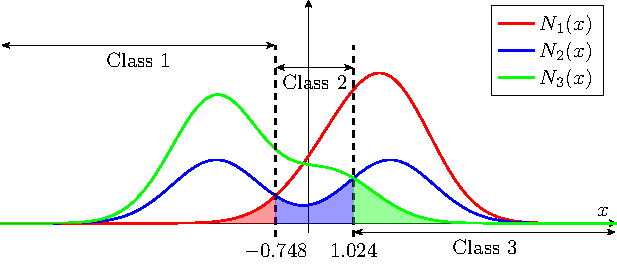
\includegraphics[width=\linewidth]{question_4a_i.pdf}
		}
		\caption{Risk in MLE}
		\label{fig:Risk_MLE}
	\end{figure}
	Thus, the optimal classifier 
	\begin{align*}
		h_{MLE} (x) = \left\{ \begin{array}{ll}
			1;& x\leq-0.748\\
			2;& -0.748<x\leq1.024\\
			3;& 1.024<x
			\end{array}
			\right.
	\end{align*}
\end{solution}

\subpart[4] Derive the optimal classifier $h_{MAP}(x)$ and provide the decision boundaries/regions, based on the Bayesian MAP estimation from data (assuming that the parameter for the class priors follows a Dirichlet distribution with parameters/pseudocounts given by (2, 2 and 2), and the mean parameter for the class conditionals follows a standard normal distribution).
\begin{solution}
	Given that 
	\begin{align*}
		y &\sim \text{Dir}\left(\pi\mid\alpha=(2,2,2)\right)\\
		x\mid y=1 &\sim \mathcal{N}(\mu_1,\sigma^2=1);\quad \mu_1\sim\mathcal{N}(0,\sigma_{0}^2=1)\\
		x\mid y=2 &\sim \mathcal{N}(\mu_2,\sigma^2=1);\quad \mu_2\sim\mathcal{N}(0,\sigma_{0}^2=1)\\
		x\mid y=3 &\sim \mathcal{N}(\mu_3,\sigma^2=1);\quad \mu_3\sim\mathcal{N}(0,\sigma_{0}^2=1)
	\end{align*}
	and by Bayesian posterior estimation we can write 
	\begin{align*}
		\pi\mid D&\sim\text{ Dir}(2+5,2+4,2+5)=\text{ Dir}(7,6,7)\\
		\mu_1\mid D&\sim \mathcal{N}(\mu_{N_1},\sigma_{N_1}^2)\\
		\mu_2\mid D&\sim \mathcal{N}(\mu_{N_2},\sigma_{N_2}^2)\\
		\mu_3\mid D&\sim \mathcal{N}(\mu_{N_3},\sigma_{N_3}^2)
	\end{align*}
	where
	\begin{align*}
		\pi_1& = \frac{7-1}{7+6+7-3}=\frac{6}{17};\quad\pi_2= \frac{6-1}{7+6+7-3}=\frac{5}{17}; &\pi_3=\frac{7-1}{7+6+7-3}=\frac{6}{17}\\
		\mu_{N_1}&=\frac{N_1\sigma_{0}^2}{N_1\sigma_{0}^2+\sigma^2}\mu_{1_{\text{ML}}}=\frac{5}{6}\times (-2.1)=-1.75;& \sigma_{N_1}^2 = 1/\left(\frac{N_1}{\sigma^2}+\frac{1}{\sigma_{0}^2}\right)=1/6\\
		\mu_{N_2}&=\frac{N_2\sigma_{0}^2}{N_2\sigma_{0}^2+\sigma^2}\mu_{2_{\text{ML}}}=\frac{4}{5}\times (0.5)=0.4;&\sigma_{N_2}^2 = 1/\left(\frac{N_2}{\sigma^2}+\frac{1}{\sigma_{0}^2}\right)=1/5\\
		\mu_{N_3}&=\frac{N_3\sigma_{0}^2}{N_3\sigma_{0}^2+\sigma^2}\mu_{3_{\text{ML}}}=\frac{5}{6}\times (1.86)=1.55;&\sigma_{N_3}^2 = 1/\left(\frac{N_3}{\sigma^2}+\frac{1}{\sigma_{0}^2}\right)=1/6
	\end{align*}
	Hence, the class prior are 
	\begin{align*}
		p(y=1)=\frac{6}{17};\quad
		p(y=2)=\frac{5}{17};\quad
		p(y=3)=\frac{6}{17}	
	\end{align*}
	and the class conditional are
	\begin{align*}
		p(x\mid y=1)=\mathcal{N}\left(-1.75,\frac{1}{6}\right);~
		p(x\mid y=2)=\mathcal{N}\left(0.4,\frac{1}{5}\right);~
		p(x\mid y=3)=\mathcal{N}\left(1.55,\frac{1}{6}\right)
	\end{align*}
	our objective to get the optimal classifier
	\begin{align*}
		h_{MAP}(x) = \argmin_{j\in\{1,2,3\}} p(y\mid x)\cdot L_{:,j}
	\end{align*} 
	if $j=1$ we have
	\begin{align*}
		p(y\mid x)\cdot L_{:,1} =p(y=2\mid x)+2p(y=3\mid x)\propto\left[\frac{5}{17}\mathcal{N}\left(0.4,\frac{1}{5}\right)+\frac{12}{17}\mathcal{N}\left(1.55,\frac{1}{6}\right)\right]:=N_1(x)
	\end{align*}
	similarly for $j=2 $ and $j=3$ we have
	\begin{align*}
		p(y\mid x)\cdot L_{:,2}& =p(y=1\mid x)+p(y=3\mid x)\propto\left[\frac{6}{17}\mathcal{N}\left(-1.75,\frac{1}{6}\right)+\frac{6}{17}\mathcal{N}\left(1.55,\frac{1}{6}\right)\right]:=N_2(x)\\
		p(y\mid x)\cdot L_{:,3}& =2p(y=1\mid x)+p(y=2\mid x)\propto\left[\frac{12}{17}\mathcal{N}\left(-1.75,\frac{1}{6}\right)+\frac{5}{17}\mathcal{N}\left(0.4,\frac{1}{5}\right)\right]:=N_3(x)
	\end{align*}
	To find the decision boundaries we know at the boundaries the risks are same(i.e., $N_i=N_j,i\neq j $). So, we can write
	\begin{align*}
		N_1(x)&=N_2(x)\Rightarrow x\approx -0.7007\\
		N_1(x)&=N_3(x)\Rightarrow x\approx -0.1\\
		N_2(x)&=N_3(x)\Rightarrow x\approx 0.9579
	\end{align*}
	Figure \ref{fig:Risk_MAP} shows the decision boundaries (minimizing expected loss under the MAP model).
	\begin{figure}[H]
		\centering
		\resizebox{0.8\linewidth}{!}{
			\centering
			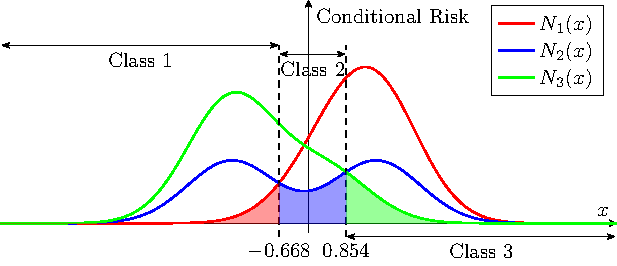
\includegraphics[width=\linewidth]{question_4a_ii.pdf}
		}
		\caption{Risk in MAP}
		\label{fig:Risk_MAP}
	\end{figure}
	Thus, the optimal classifier 
	\begin{align*}
		h_{MAP} (x) = \left\{ \begin{array}{ll}
			1;& x\leq-0.7007\\
			2;&-0.7007<x\leq0.9579\\
			3;& 0.9579<x
		\end{array}
		\right.
	\end{align*}
\end{solution}

\subpart[1] Is there any $x \in \mathbb{R}$ that is differently classified by the above two classifiers? 
\begin{solution}
	Yes there exist $x\in\mathbb{R}$ that is differently classified by the above two classifiers.
	For $x\in[-0.748,-0.7007]$ the MLE model classifies as class 2 whereas MAP model classifies as class 1. Similarly for $x\in[0.9579,1.024]$ the MLE model classifies as class 2, where as the MAP model classifies as class-3.
\end{solution}
\end{subparts}

\part[2] Consider a classification problem in which the loss incurred on mis-classifying an input vector from class $C_k$  as $C_j$ is given by loss matrix entry $L_{kj}$, and for which the loss incurred in selecting the reject option is $\psi$. Find the decision criterion that will give minimum expected loss, and then simplify it for the case of 0-1 loss (i.e., when $L_{kj} = \mathbbm{1}_{k \ne j}$).
\begin{solution}
\end{solution}
%\newpage
\end{parts}


\question[15] [{\sc Let's roll up your coding sleeves...}]
\red{(Note: You should follow the ``General Instructions'' above on how to submit your python notebook with output/results, as well as the code source files, to get full credit for this programming question.)}\\
Given a feature vector $x \in \mathbb{R}^d$ and class labels $C \in \{c_1, \dots, c_k\}$, the Bayes classifier assigns $x$ to the class with maximum posterior probability:
\[
h(x) = \arg\max_{c \in \{c_1, \dots, c_k\}} P(C=c \mid X=x).
\]

The Naive Bayes classifier assumes conditional independence of features given the class, i.e. 
\[
P(X=x \mid C=c) = \prod_{j=1}^d P(X_j = x_j \mid C=c),
\]
You are supposed to build Bayes classifiers that model each class using multivariate Gaussian density functions for the datasets assigned to you (under assumptions below and employing MLE approach to estimate class prior/conditional densities). This assignment is focused on handling and analyzing data using interpretable classification models, rather than aiming solely for the best classification accuracy. 
    
Build classification models for all these Case numbers (you may refer to the Chapter 2 of the book ``Pattern Classification" by David G. Stork, Peter E. Hart, and Richard O. Duda):
\begin{enumerate}
    \item[Case 1:] Bayes classifier with the same Covariance matrix for all classes.
    \item[Case 2:] Bayes classifier with different Covariance matrix across classes.
    \item[Case 3:] Naive Bayes classifier with the Covariance matrix $S = \sigma^2 \mathbf{I}$ same for all classes.
    \item[Case 4:] Naive Bayes classifier with $S$ of the above form, but being different across classes.
\end{enumerate}
    
Refer to the provided dataset for each group, which can be found  \href{https://drive.google.com/drive/folders/1YwSDijf-LOF3HZwSBoMc5R02TH_o12s3?usp=sharing}{here}. Each dataset includes 2D feature vectors and their corresponding class labels. There are two different datasets available:
\begin{enumerate}
    \item Linearly separable data.
    \item Non-linearly separable data.
\end{enumerate}
There are 41 folders in each dataset, but you need to look at only one folder -- {\bf the folder number assigned to you} being $RollNo\%41 + 1$.
    
\textbf{Plots/answers Required}:
For your assignment, you need to provide the following plots/answers (refer to the "Sample Plots" folder: \href{https://drive.google.com/drive/folders/1YwSDijf-LOF3HZwSBoMc5R02TH_o12s3?usp=sharing}{link}):
    
\begin{parts}
\part[4] The plot of Gaussian pdfs for all classes estimated using the train data (train.txt). (4 Cases $\times$ 2 Datasets = 8 plots in one page)
%\newpage
\begin{solution}
	\begin{figure}[H]
		\centering
		\resizebox{.6\linewidth}{!}{
			\centering
			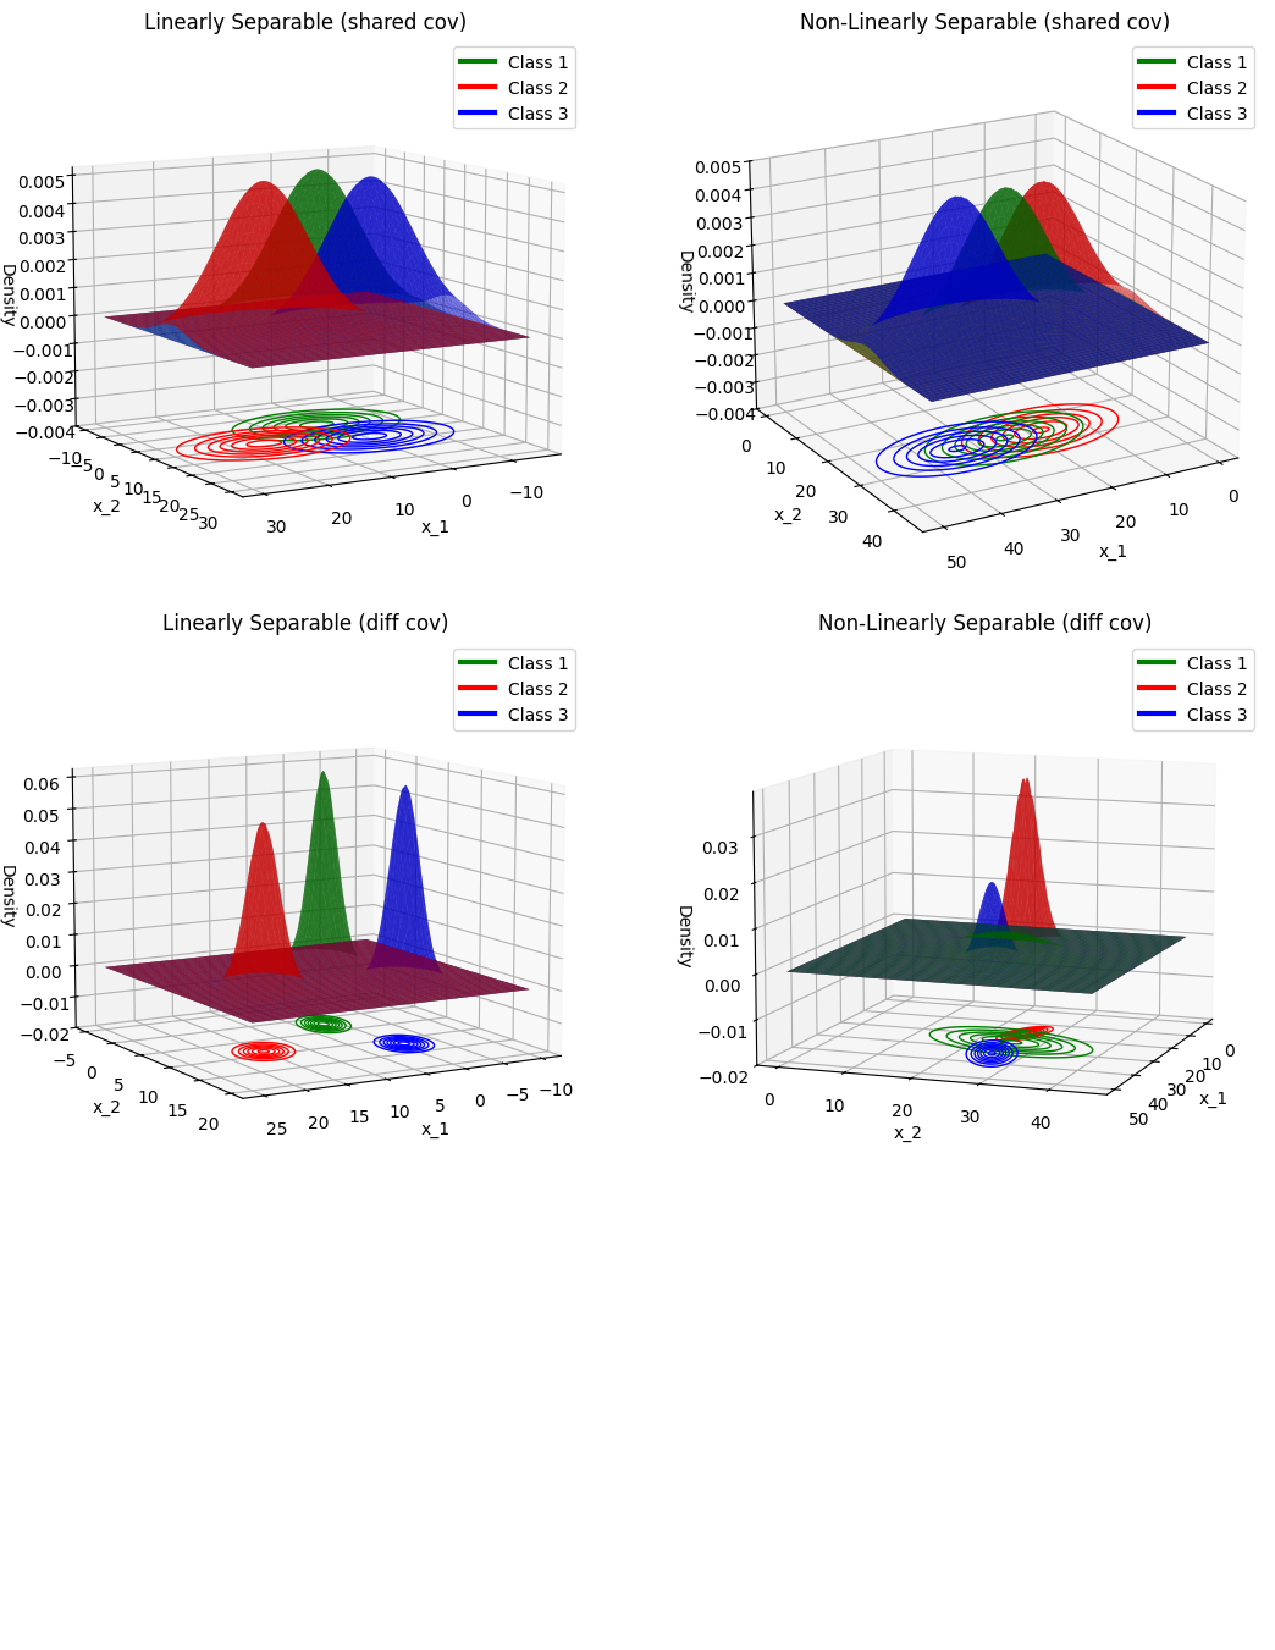
\includegraphics[width=\linewidth]{plots/pdf_case1.pdf}
		}
		\caption{Risk in MAP}
		\label{fig:pdf_1}
	\end{figure}
\end{solution}

\part[4] The classifiers, specifically their decision boundary/surface as a 2D plot along with training points marked in the plot (again 8 plots in one page).
\begin{solution}
	\begin{figure}[H]
		\centering
		\resizebox{.7\linewidth}{!}{
			\centering
			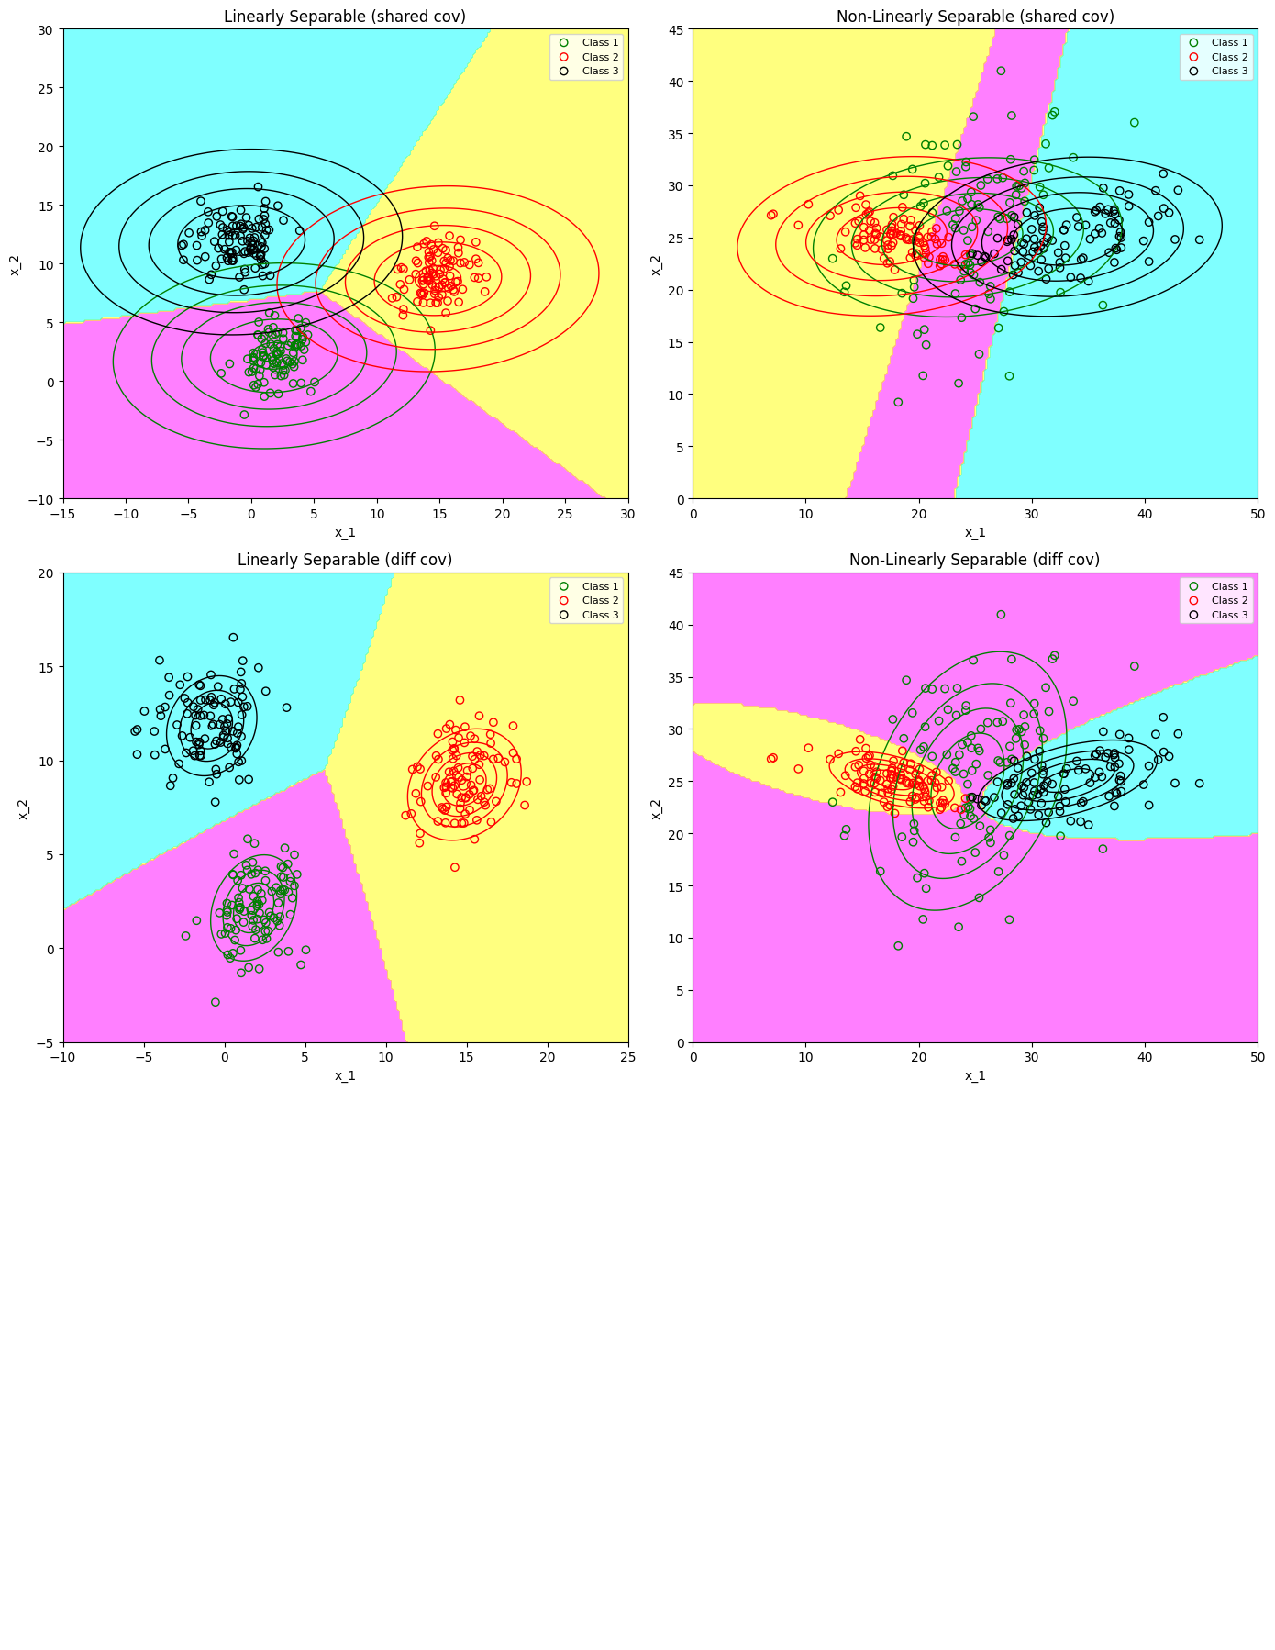
\includegraphics[width=\linewidth]{plots/decision_boundary_bayes_classifier.pdf}
		}
		\caption{Decision Boundary}
		\label{fig:decision_boundary}
	\end{figure}
\end{solution}

\part[1] Report the error rates for the above classifiers (four classifiers on the two datasets as a 4 × 2 table, with appropriately named rows and columns).
\begin{solution}
	Error rate on test data:
	\begin{center}
		\begin{tabular}{|c|c|c|}
			\hline
			Bayes Classifier & Linearly Separable & Non-Linearly Separable \\
			\hline
			Shared Covariance & 0 & 0.233 \\
			\hline
			Different Covariance & 0 & 0.0267 \\
			\hline
		\end{tabular}
	\end{center}
\end{solution}

\part[1] Answer briefly on whether we can use the most general ``Case 2'' for all datasets? If not, answer when a simpler model like ``Case 1'' is preferable over ``Case 2''? 
\begin{solution}
	No we can't always use the case-2. It requires estimating more parameters(i.e. different covariance matrices) and can overfit when the data is limited. Whereas case-1 is simpler mode is preferable when the class covariance are similar, data is roughly linearly separable, or/and the training set is small.
\end{solution}

\part[5] Ensure that the properly running code files that generates the above plots, etc., are submitted according to the detailed ``General Instructions'' in the beginning of this document.
%\begin{solution}
%\end{solution}
%\newpage
\end{parts}
    
\textbf{(Not)Allowed Libraries:}
You are not allowed to use any inbuilt functions for building the model or classification using the model. However, you can use inbuilt functions/libraries for plotting and other purposes.


\question
{\sc [Self Declaration]}\\
I, \underline{Ritabrata Mandal} ,swear on my honour that I have prepared and written the answers for this assignment and associated code by myself and have not copied it from the internet, any LLM's output, or other students.
\end{questions}
\end{document}

